\section{Еквівалентні перетворення}

Існує достатня умова оптимальності нечіткої розмітки. Якщо нечітка розмітка
$(\alpha, \beta)$ задовольняє умовам
\begin{equation}
    \label{eqn:trivial_optim_cond}
    \begin{cases}
      q_t(k)< \max\limits_{\ell \in K} q_t(\ell) , & \implies \alpha_t(k)=0,\\
      g_{tt'}(k,k')<\max\limits_{\ell\in K, \ell'\in K} g_{tt'}(k,k'), & \implies
        \beta_{tt'}(k,k')=0,
    \end{cases}
  \end{equation}
то розмітка є оптимальною нечіткою розміткою. Дана умова є дуже строгою,
тому лише невеликий клас задач підпадає під цю умову. Задачі, які задовольняють
цю умову, називаються тривіальними. Можна послабити
умову \eqref{eqn:trivial_optim_cond}, використовуючи концепцію еквівалентних
перетворень \cite{SchlGig_1_usim2007, Shlezinger_synt}.
Дві задачі $(q^1,g^1)$ та $(q^2,g^2)$ нечіткої розмітки, що визначені на однаковій множині об'єктів
$T$ та однаковій множині міток $K$, називаються еквівалентними (позначаємо $(q^1,g^1) \sim (q^2,g^2)$),
якщо якості кожної нечіткої розмітки однієї задачі дорівнюють якості цієї ж
нечіткої розмітки іншої задачі. Також відомо, що для кожної задачі нечіткої
розмітки $(q,g)$ існує тривіальний еквівалент. Задача $(q^*,g^*)$, за якої значення
\begin{equation}
   E(q',g') = \sum\limits_{tt'\in\Gamma}\max\limits_{k\in K, k'\in K}g'_{tt'}(k,k')+
    \sum\limits_{t\in T}\max\limits_{k\in K} q'_t(k),
\end{equation}
є мінімальним з можливих, називається потужністю класу еквівалентності
\begin{equation}
    (q^*,g^*) = \argmin\limits_{(q',g')\sim (q,g)} E(q',g').
   \end{equation}

Дві задачі розмітки із якостями $q^1$, $g^1$ і $q^2$, $g^2$ відповідно
є еквівалентними тоді й тільки тоді, коли існує такий набір чисел
$\varphi_{tt'}(k), t\in T, t'\in N(t), k\in K$, який задовольняє систему рівностей
\begin{equation*}
    \begin{cases}
      q^1_t(k) = q^2_t(k) - \sum\limits_{t'\in N(t)} \varphi_{tt'}(k), & t\in T, k\in K,\\
      g^1_{tt'}(k,k') = g^2_{tt'}(k,k') + \varphi_{tt'}(k) + \varphi_{t't}(k), &
        tt'\in\Gamma, k\in K, k'\in K.
    \end{cases}
  \end{equation*}
Таким чином, потужність еквівалентно трансформованої задачі може бути
явно виражена як функція $\varphi$
\begin{equation}
    \label{eqn:trivial_power}
    E(\varphi) = \sum\limits_{tt'\in\Gamma}\max\limits_{k\in K, k'\in K}[ g_{tt'}(k,k')
    + \varphi_{tt'}(k) + \varphi_{t't}(k)] +
    \sum\limits_{t\in T}\max\limits_{k\in K}[ q_t(k) - \sum\limits_{t'\in N(t)} \varphi_{tt'}(k)],
   \end{equation}
і зведення задачі до тривіальної може бути виконано шляхом мінімізації \eqref{eqn:trivial_power}
без жодних обмежень на $\varphi$.

\section{Представлення у вигляді задачі лінійного програмування}

Представимо $(\max,+)$ задачу розмітки як задачу
лінійного програмування \cite{Werner:2010, savchynskyy}. Для кожної
вершини $(t,k)$, $t\in T$, $k\in K$ введемо число $\alpha_t(k)\in [0,1]$.
Для кожного ребра $(t,k),(t',k')$, $t\in T$, $k\in K$, $t'\in N_t$, $k'\in K$, яке поєднує мітки
$k$ і $k'$ в сусідніх об'єктах $t$ і $t'$, введемо число $\beta_{tt'}(k,k')$.

Елементи вектору $\alpha_t(k)$, що відповідають вершинам, мають бути узгодженими з
з розміткою $k$, тобто, якщо виконується $\alpha_t(k^*)=1$ для якоїсь мітки
$k^*\in K$, то має також виконуватися $k(t)=k^*$. За визначенням для задання розмітки
$k\in K^T$ потрібно в кожному об'єкті $t\in T$ обрати єдину мітку $k\in K$.
Тому на елементи вектора $\alpha_t(k)$ накладаються обмеження однозначності для
кожної вершини в об'єкті
\begin{equation*}
   \sum\limits_{k \in K} \alpha_t(k)=1,  t\in T.
 \end{equation*}
Відмітимо, що для випадку $\alpha_t(k)\in \{0,1\}$ ця умова означає
вибір єдиної мітки в об'єкті, бо для обраної мітки $k^*$ буде виконуватися
$\alpha_t(k^*)=1$, а для всіх інших міток $k'\in K:k'\neq k^*$
\begin{equation*}
  \sum\limits_{k \in K, k\neq k^*} \alpha_t(k)=0.
\end{equation*}

\begin{figure}[h]
  \centering
  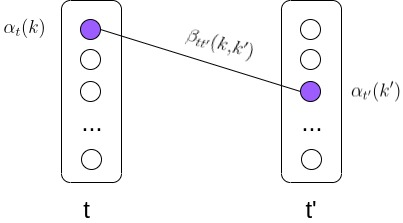
\includegraphics[width=0.5\textwidth]{images/coupling_constr.jpg}
  \caption{Поєднуючі обмеження}
  \label{fig:coupling_constr}
\end{figure}

Нехай об'єкт $t'\in T$ є сусідом об'єкту $t\in T$, тобто $tt'\in \Gamma$. Якщо
в об'єкті $t'$ була обрана мітка $k'\in K$, то має існувати таке ребро, яка поєднує
якусь із вершин об'єкту $t' \in T$ і вершину $(t',k')$, тобто
\begin{equation*}
  \sum\limits_{k\in K}\beta_{tt'}(k,k')=\alpha_{t'}(k'), \forall t\in T, t'\in N_t, k'\in K.
\end{equation*}
Обмеження такого виду називають поєднуючими (рис. \ref{fig:coupling_constr}).
Якщо $\beta_{tt'}(k,k')\in \{0,1\}$, $\forall tt'\in\Gamma$, $k\in K$, $k'\in K$,
то з цих обмежень також випливає, що між двома сусідніми об'єктами $tt'\in\Gamma$ може бути
обране лише одне ребро, тобто додатково накладаються обмеження однозначності
для ребер між парами сусідніх об'єктів
\begin{equation*}
  \sum\limits_{k \in K, k'\in K} \beta_{tt'}(k,k')=1, \forall tt'\in\Gamma.
\end{equation*}
Отримали наступну множину обмежень
\begin{equation*}
  L \equiv
  \begin{cases}
    \sum\limits_{k' \in K} \beta_{tt'}(k,k') = \alpha_t(k), & t\in T, k\in K, t'\in N_t,\\
    \sum\limits_{k \in K} \alpha_t(k)=1, & t\in T,\\
    \beta_{tt'}(k,k')\geq 0, & tt'\in \Gamma, k\in K, k'\in K,\\
    \alpha_t(k)\geq 0, & t\in T, k\in K.
  \end{cases}
\end{equation*}
Позначимо множину всіх вершин і ребер графу як $I$
\begin{equation*}
  I = \{(t,k):t\in T, k\in K\}\cup\{((t,k),(t',k')):t\in T, t'\in\Gamma, k\in K, k'\in K\}.
\end{equation*}
Позначимо множину всіх якостей задачі як $\theta$
\begin{equation*}
  \theta = \{q_t(k):t\in T, k\in K\}\cup\{g_{tt'}(k,k'):t\in T, t'\in\Gamma, k\in K, k'\in K\}.
\end{equation*}
Множину всіх чисел $\alpha, \beta$ позначимо як
\begin{equation*}
  \mu = \{\alpha_t(k):t\in T, k\in K\}\cup\{\beta_{tt'}(k,k'):t\in T, t'\in\Gamma, k\in K, k'\in K\}.
\end{equation*}
Тоді $(\max,+)$ задачу розмітки можна представити як задачу лінійного програмування
\begin{equation*}
  \max\limits_{\mu\in L\cap \{0,1\}}\langle\theta,\mu\rangle.
\end{equation*}
Легко побачити, що виконується рівність
\begin{equation*}
  \label{eqn:max-eq-max}
  \max_{k\in K^T} G(k) = \max\limits_{\mu\in L\cap \{0,1\}}\langle\theta,\mu\rangle.
\end{equation*}
Розпишемо скалярний добуток правої частини рівності \eqref{eqn:max-eq-max} у явному вигляді
\begin{equation}
  \label{eqn:linear_prog}
  \begin{gathered}
  \max\limits_{\mu\in L\cap \{0,1\}}\langle\theta,\mu\rangle = \\
  =
  \max\limits_{\mu\in L\cap \{0,1\}} \left[ \sum\limits_{t\in T}\sum\limits_{k\in K} \alpha_t(k)\cdot q_t(k) +
  \sum\limits_{tt'\in \Gamma}\sum\limits_{k,k'\in K} \beta_{tt'}(k,k')\cdot g_{tt'}(k,k') \right].
  \end{gathered}
\end{equation}
Дуалізуємо поєднуючі обмеження задачі \eqref{eqn:linear_prog}. Новий доданок буде
мати вигляд
\begin{equation}
  \label{eqn:relax}
  \sum\limits_{t\in T}\sum\limits_{t'\in N_t}\sum\limits_{k\in K} \varphi_{tt'}(k)\cdot \left[ \sum\limits_{t'\in T}\beta_{tt'}(k,k')-\alpha_t(k) \right],
\end{equation}
де змінні $\varphi_{tt'}(k)\in \mathbb{R}$, $t\in T$, $t'\in N_t$, $k\in K$ є двоїстими. В подальшому будемо
називати їх потенціалами.
Перепишемо функцію \eqref{eqn:linear_prog} з урахуванням нового доданку \eqref{eqn:relax}, в якому
розкриємо дужки
\begin{gather*}
  \langle\theta^{\varphi},\mu\rangle = \sum\limits_{t\in T}\sum\limits_{k\in K} \alpha_t(k)\cdot q_t(k)+
  \sum\limits_{tt'\in \Gamma}\sum\limits_{k,k'\in K} \beta_{tt'}(k,k')\cdot g_{tt'}(k,k')+\\
  \sum\limits_{t\in T}\sum\limits_{t'\in N_t}\sum\limits_{k\in K} \varphi_{tt'}(k)\cdot
  \sum\limits_{t'\in T}\beta_{tt'}(k,k') - \sum\limits_{t\in T}\sum\limits_{t'\in N_t}\sum\limits_{k\in K} \varphi_{tt'}(k)\cdot \alpha_t(k).
\end{gather*}
Згрупуємо доданки в такому порядку: перший і останній, другий і третій
\begin{equation}
  \label{eqn:reparam}
  \begin{gathered}
  \langle\theta^{\varphi},\mu\rangle = \sum\limits_{t\in T}\sum\limits_{k\in K} \alpha_t(k)\cdot \left[ q_t(k)- \sum\limits_{t'\in N_t} \varphi_{tt'}(k) \right]+\\
  \sum\limits_{tt'\in \Gamma}\sum\limits_{k,k'\in K} \beta_{tt'}(k,k')\cdot \left[g_{tt'}(k,k') + \varphi_{tt'}(k) + \varphi_{t't}(k') \right].
  \end{gathered}
\end{equation}
Введемо позначення для репараметризованої якості мітки $k\in K$ в
об'єкті $t\in T$
\begin{equation}
  \label{eqn:reparam_unary}
  q^{\varphi}_t(k) = q_t(k) - \sum\limits_{t'\in N_t} \varphi_{tt'}(k).
\end{equation}
Репараметризована якість у вершині отримується шляхом віднімання потенціалів,
що виходять з даної вершини $(t,k)$, $t\in T$, $k\in K$ в усі сусідні об'єкти
$t'\in N_t$, від вихідної якості в даній вершині. Введемо позначення для
репараметризованої якості вибору пари міток $k\in K$, $k'\in K$ у двох сусідніх
об'єктах $tt'\in\Gamma$
\begin{equation}
  \label{eqn:reparam_binary}
  g^{\varphi}_{tt'}(k,k') = g_{tt'}(k,k') + \varphi_{tt'}(k) + \varphi_{t't}(k'),
\end{equation}
тобто репараметризована якість за вибір ребра $((t,k),(t',k')$, $t\in T$, $t'\in N_t$, $k\in K, k'\in K)$
отримується шляхом додавання потенціалів, що виходять в об'єкти $t$ і $t'$, які дане ребро поєднує,
до вихідної якості даного ребра.
Використаємо позначення у виразі \eqref{eqn:reparam}
\begin{gather*}
  \langle\theta^{\varphi},\mu\rangle =  \sum\limits_{t\in T}\sum\limits_{k\in K} \alpha_t(k)\cdot q^{\varphi}_t(k)+
  \sum\limits_{tt'\in \Gamma}\sum\limits_{k,k'\in K} \beta_{tt'}(k,k')\cdot g^{\varphi}_{tt'}(k,k').
\end{gather*}

\textbf{Твердження.}
Після перетворень \eqref{eqn:reparam_unary} та \eqref{eqn:reparam_binary} значення
штрафної функції не зміниться для будь-якої розмітки $k\in K^T$.

Для доведення цього твердження запишемо штрафну функцію з репараметризованими
якостями
\begin{gather*}
  G^{\varphi}(k) =  \sum\limits_{t\in T} q^{\varphi}_t(k)+
  \sum\limits_{tt'\in \Gamma} g^{\varphi}_{tt'}(k,k')=\\
  =\sum\limits_{t\in T}  \left[ q_t(k)- \sum\limits_{t'\in N_t} \varphi_{tt'}(k) \right]
  +\sum\limits_{tt'\in \Gamma} \left[g_{tt'}(k,k') + \varphi_{tt'}(k) + \varphi_{t't}(k') \right].
\end{gather*}
Розкриємо дужки в останньому виразі
\begin{gather*}
  G^{\varphi}(k) =  \sum\limits_{t\in T} q_t(k)-\sum\limits_{t\in T}\sum\limits_{t'\in N_t}\varphi_{tt'}(k)+\\
  +\sum\limits_{tt'\in \Gamma}g_{tt'}(k,k')+\sum\limits_{tt'\in \Gamma}\left[ \varphi_{tt'}(k) + \varphi_{t't}(k')\right]=G(k),
\end{gather*}
тому що перший і третій доданки в сумі дають $G(k)$, а другий і четвертий доданки в сумі дорівнюють нулю.
Отримали
\begin{equation*}
  G^{\varphi}(k) = G(k), \forall k\in K^T.
\end{equation*}
Маємо двоїсту задачу, цільову функцію якої будемо мінімізувати
\begin{equation}
  \min_{\Phi}\max_{\mu\in L\cap \{0,1\}}\langle\theta,\mu\rangle,
\end{equation}
де
\begin{equation}
  \Phi = \{\varphi_{tt'}(k)\in\mathbb{R}|t\in T, t'\in N_t, k\in K\}.
\end{equation}
Отримали остаточний вигляд двоїстої цільової функції, яку будемо мінімізувати
по набору двоїстих змінних $\varphi$.

\section{Властивості задачі}

Задача розмітки називається супермодулярною, якщо існує таке відношення
$n:T\times K\rightarrow {1,\dots, \left\lvert K\right\rvert } $,
що для будь-яких значень $k\in K$, $k'\in K$, $\ell \in K$, $\ell'\in K$ і $tt'\in \Gamma$ з умов
$n_t(k)\geq n_t(\ell)$ та $n_t'(k')\geq n_t'(\ell')$ випливає
\begin{equation*}
    g_{tt'}(k,k') + g_{tt'}(\ell,\ell')\geq g_{tt'}(k,\ell') + g_{tt'}(\ell,k').
   \end{equation*}
Ребра $((t,k),(t',k')))$ і $((t,\ell),(t',\ell'))$ називають паралельними,
а ребра $((t,\ell),(t',k'))$ називають перехресними, тому наведену нерівність
можна інтерпретувати наступним чином: сума якостей паралельних ребер є не гіршою
за суму якостей перехресних ребер (рис. \ref{fig:submodularity_example}). При цьому на функцію $q$ обмежень не накладається.

Розглядаються два випадки. Якщо задача є супермодулярною і відображення $n$ відоме,
задача називається супермодулярною з відомою впорядкованістю. Коли відомо, що існує таке
$n$, проте саме відображення невідоме, задача називається супермодулярною з
невідомою впорядкованістю.
\begin{figure}[h]
  \centering
  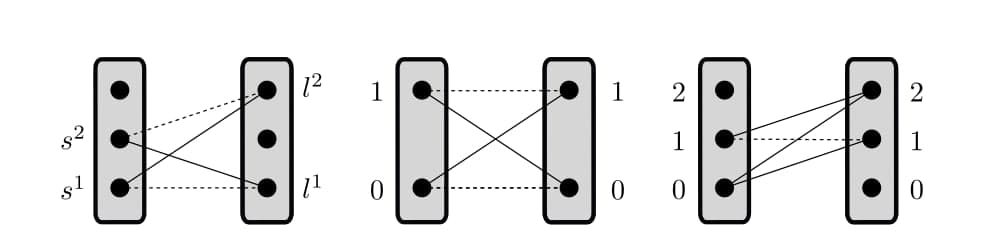
\includegraphics[width=1\textwidth]{images/submodularity_ilustr.jpg}
  \caption{Властивість супермодулярності для ребер \cite{ishikawa}}
  \label{fig:submodularity_example}
\end{figure}
Пряма перевірка супермодулярності є досить складною задачею. Для
однієї пари об'єктів $tt'\in \Gamma$ складність перевірки
$\mathcal{O}(|K^2|)$, а перевірка всієї задачі на супермодулярність ---
$\mathcal{O}(|K^2|\cdot |\Gamma|)$. Така перевірка стає проблемою у випадку,
коли множини $T$, $K$ досить великі, що не є рідкістю на практиці.

Досить багато штрафів можна представити у вигляді супермодулярних
функцій. Наведемо деякі з них.

\textbf{Модель Ізінга}
\begin{equation*}
  g_{tt'}(k,k') = \lambda_{tt'}\cdot \llbracket t \neq t' \rrbracket
 \end{equation*}
для деяких констант $\lambda_{tt'}$, $tt'\in\Gamma$, $k\in K$, $k'\in K$, $\left\lvert K\right\rvert = 2$.
Можна показати, що використовуючи репараметризацію,
будь-яку бінарну функцію якостей можна перетворити в форму моделі Ізінга.

\textbf{Модель Поттса} є узагальненням моделі Ізінга для випадку, коли $|K|\geq 2$.
Бінарні якості мають аналогічний вигляд
\begin{equation*}
  g_{tt'}(k,k') = \lambda_{tt'}\cdot \llbracket t \neq t' \rrbracket.
\end{equation*}

Моделі Потса та Ізінга часто використовуються, коли задачі мають дискретний
характер. Іноді ж потрібно на лише штрафувати за неправильну мітку, а штрафувати
за за неправильну мітку пропорційно відстані до правильної. Для цього також
необхідно, щоб на множині $K$ існував порядок.

\textbf{Пропорційні відстані}
\begin{equation*}
  g_{tt'}(k,k') = |k - k'|^n, n\geq 2.
\end{equation*}
Прикладами задач, де можуть застосовуватися штрафи такого типу: сегментація,
стереозір, постеризація, домальовування (inpainting), та багато інших.

\textbf{Твердження.}
Сума 2 супермодулярних функцій $g^1_{tt'}(k,k')$ та $g^2_{tt'}(k,k')$ також є супермодулярною
\begin{equation*}
  g_{tt'}(k,k')=g^1_{tt'}(k,k')+g^2_{tt'}(k,k').
\end{equation*}

\textbf{Твердження.}
Репараметризація не впливає на властивість супермодулярності, тобто, якщо функція була
супермодулярною, після репараметризації вона також буде супермодулярною.
Розглянемо довільну пару сусідів $tt'\in\Gamma$ і функцію якостей $g_{tt'}(k,k'), k\in K, k'\in K$.
Якщо $g_{tt'}(k,k')$ є супермодулярною, то
\begin{equation}
  g^{\varphi}_{tt'}(k,k')=g_{tt'}(k,k') + \varphi_{tt'}(k) + \varphi_{t't}(k')
\end{equation} також є супермодулярною.
Треба перевірити чи виконується нерівність
\begin{equation}
  g^{\varphi}_{tt'}(k,k') + g^{\varphi}_{tt'}(\ell,\ell')\geq g^{\varphi}_{tt'}(k,\ell') + g^{\varphi}_{tt'}(\ell,k').
\end{equation}
Розпишемо репараметризовані якості
\begin{gather*}
  g_{tt'}(k,k') + \varphi_{tt'}(k) + \varphi_{t't}(k') + g_{tt'}(\ell,\ell') + \varphi_{tt'}(\ell) + \varphi_{t't}(\ell') \geq \\
  \geq g_{tt'}(k,\ell') + \varphi_{tt'}(k) + \varphi_{t't}(\ell') + g_{tt'}(\ell,k') + \varphi_{tt'}(\ell) + \varphi_{t't}(k').
\end{gather*}
Перенесемо всі доданки з $\varphi$ в одну частину
\begin{gather*}
  g_{tt'}(k,k') + g_{tt'}(\ell,\ell') \geq g_{tt'}(k,\ell') + g_{tt'}(\ell,k') + \\
  + [\varphi_{tt'}(k) + \varphi_{t't}(\ell')  + \varphi_{tt'}(\ell) + \varphi_{t't}(k')-\\
   -\varphi_{tt'}(k) - \varphi_{t't}(k') - \varphi_{tt'}(\ell) - \varphi_{t't}(\ell')].
\end{gather*}
Видно, що всі доданки з $\varphi$ скорочуються і потрібна рівність виконується.
